\section{Data and simulated samples}\label{chap6:datatsets}

The data sets, triggers, pile-up reweighting, lepton identification and isolation used in this analysis are the same as the 125\GeV mass Higgs boson measurement and are described in Sec.~\ref{chap5:dataset}.

Also, the same MC simulations are used for the background processes, the only exception being the \dyll background. Given that this analysis aims to probe regions of phase space where the \dyll contribution is very small, like in the high transverse mass region, the usage of a simulation of the inclusive \dyll process leads to large uncertainties due to the limited simulation statistics in the sample. To partially overcome this issue the \textsc{MadGraph5\_aMC@NLO} generator is used with LO QCD accuracy, matching together events with up to four jets in addition to the vector boson with the MLM matching scheme~\cite{Alwall:2007fs}, in order to generate different \dyll samples in restricted portions of the phase space defined by the $H_\mathrm{T}$ variable, i.e. the scalar sum of all the partons \pt in the event. 
%For $H_\mathrm{T}< 100$\GeV the inclusive simulation is used, while different samples are used for higher values of $H_\mathrm{T}$. 
The samples are merged using the parton level information, and a smooth transition between different $H_\mathrm{T}$ regions is achieved, as shown in Fig.~\ref{fig:DY_HT}. The \dyll LO cross section obtained from the simulation is scaled using a LO to NNLO $k$-factor of 1.23.

\begin{figure}[htbp]
\centering
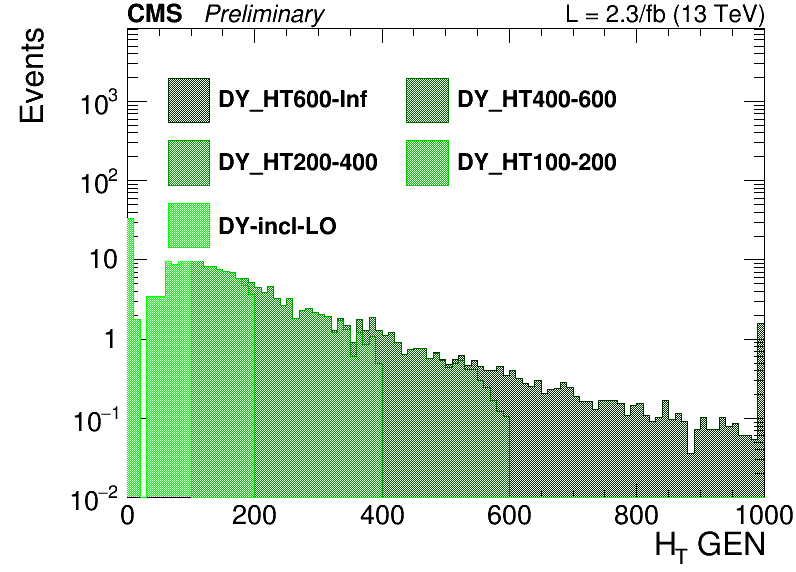
\includegraphics[width=0.5\textwidth]{images/13TeV/log_c_incl_HTGen.png}
\caption{
    Generator level $H_\mathrm{T}$ distribution for the merged \dyll (denoted as DY in the legend) sample.}
    \label{fig:DY_HT}
\end{figure}

In order to perform a search of resonances in a large part of the mass spectrum, several signal samples for the ggH\footnote{The ggH notation is used for the gluon-gluon fusion production mode, even in the cases where a non-SM Higgs boson is created through this mechanism.} and VBF mechanisms have been generated corresponding to different resonance masses in the range between 200\GeV and 1\TeV. The signal width for each mass point corresponds to the one expected for a SM Higgs-like boson at that mass (see Fig.~\ref{fig:width}). The samples are produced with a mass step of 50\GeV from 250 to 800\GeV and of 100\GeV from 800 to 1000\GeV. A finer stepping is used between 200 and 250\GeV. All signal samples are generated with the \textsc{Powheg V2} generator, interfaced with the \textsc{JHUGen v6.2.8} generator, which handles the decay of the scalar resonance to $\mathrm{W W}\to2\ell2\nu$.

The interference effects among $\mathrm{gg\to X \to WW}$, $\mathrm{gg\to WW}$ and $\mathrm{gg\to H \to WW}$ are evaluated using the  \textsc{MCFM} and \textsc{JHUGen} generators, as implemented in the MELA (Matrix Element Likelihood Approach) framework~\cite{JHUGen}. Details about the interference effects are given in Sec.~\ref{chap6:AnalysisStrategy}.
